% =====================================================================
% PLANTILLA BASE - Trabajos académicos Universidad de Córdoba
% Reemplaza los campos entre <> y borra los comentarios de ejemplo.
% Compilar con: pdflatex x3
% =====================================================================

\documentclass[12pt,letterpaper]{article}

\usepackage[utf8]{inputenc}
\usepackage[T1]{fontenc}
% \usepackage[spanish,es-tabla]{babel}  % Descomentar SOLO si el entorno
                                        % tiene el archivo de idioma español.
                                        % Si no, usar los \renewcommand de abajo.
\usepackage[margin=2.54cm]{geometry}
\usepackage{setspace}
\usepackage{mathptmx}
\usepackage{booktabs}
\usepackage{hanging}
\usepackage{array}
\usepackage{longtable}
\usepackage{float}
\usepackage{tikz}
\usetikzlibrary{positioning, arrows.meta, shapes}
\usepackage[hidelinks]{hyperref}
\usepackage{xurl}   % IMPORTANTE: va después de hyperref. Evita que las
                    % URLs largas se salgan del margen.

\pagestyle{plain}   % Paginación en el pie, sin encabezados.
\color{black}
\doublespacing

% Nombres en español (necesarios si no se carga babel)
\renewcommand{\contentsname}{Índice}
\renewcommand{\listtablename}{Índice de tablas}
\renewcommand{\listfigurename}{Índice de figuras}
\renewcommand{\tablename}{Tabla}
\renewcommand{\figurename}{Figura}

\begin{document}

% ============== PORTADA ==============
\begin{titlepage}
\centering
\vspace*{1cm}
{\Large \textbf{UNIVERSIDAD DE CÓRDOBA}}\\[0.3cm]
{\large FACULTAD DE INGENIERÍA}\\[0.2cm]
{\large PROGRAMA DE INGENIERÍA DE SISTEMAS}\\[0.2cm]
{\large SEDE MONTERÍA}\\[1.7cm]
\rule{\textwidth}{0.5pt}\\[0.3cm]
{\Huge \textbf{<NOMBRE DE LA ACTIVIDAD>}}\\[0.4cm]
{\LARGE \textbf{<Título del trabajo>}}\\[0.3cm]
\rule{\textwidth}{0.5pt}\\[0.5cm]
{\large \textit{<Una oración que resuma de qué trata el trabajo>}}\\[2.5cm]
\begin{minipage}{0.45\textwidth}
\begin{flushleft}
\textbf{Presentado por:}\\[0.2cm]
<Nombre 1>,\\
<Nombre 2>,\\
<Nombre 3>
\end{flushleft}
\end{minipage}\hfill
\begin{minipage}{0.45\textwidth}
\begin{flushright}
\textbf{Docente:}\\[0.2cm]
<Nombre del docente>\\
\textit{<Nombre de la asignatura>}
\end{flushright}
\end{minipage}\\[2.5cm]
\vfill
Montería, Córdoba\\
<Mes> de <Año>
\end{titlepage}
\newpage

\setcounter{tocdepth}{3}
\tableofcontents
\listoftables
\listoffigures
\newpage

% ============== CUERPO ==============
% Patrón obligatorio: sección sin numerar + entrada en el índice.

\section*{Introducción}
\addcontentsline{toc}{section}{Introducción}

<Texto de la introducción.>

\newpage
\section*{<Sección>}
\addcontentsline{toc}{section}{<Sección>}

\subsection*{<Subsección>}
\addcontentsline{toc}{subsection}{<Subsección>}

<Texto. Menciona siempre las tablas y figuras: "como se resume en la
Tabla \ref{tab:ejemplo}".>

% ---------- PATRÓN DE TABLA ----------
% El bloque \endfirsthead / \endhead evita que el índice de tablas
% duplique la entrada cuando la tabla ocupa más de una página.

\begin{longtable}{>{\raggedright\arraybackslash}p{0.28\textwidth} >{\raggedright\arraybackslash}p{0.62\textwidth}}
\caption{<Título de la tabla>}\label{tab:ejemplo}\\
\toprule
\textbf{<Columna 1>} & \textbf{<Columna 2>} \\
\midrule
\endfirsthead
\multicolumn{2}{l}{\small\textit{Continuación de la tabla}}\\
\toprule
\textbf{<Columna 1>} & \textbf{<Columna 2>} \\
\midrule
\endhead
<Celda> & <Celda> \\
\addlinespace
<Celda> & <Celda> \\
\bottomrule
\end{longtable}

% ---------- PATRÓN DE FIGURA ----------
% Capas apiladas: legibles y sin texto superpuesto.
% Evitar círculos concéntricos, que casi siempre encabalgan el texto.

\begin{figure}[H]
\centering
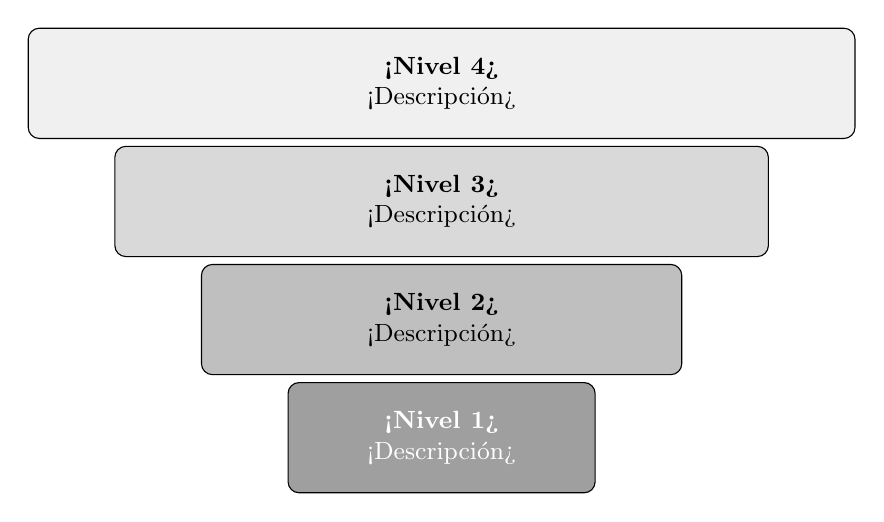
\begin{tikzpicture}[
    every node/.style={font=\small, align=center},
    capa/.style={draw, rounded corners, minimum height=1.4cm}
]
\node[capa, fill=gray!12, minimum width=10.5cm] at (0,3.6) {\textbf{<Nivel 4>}\\<Descripción>};
\node[capa, fill=gray!30, minimum width=8.3cm]  at (0,2.1) {\textbf{<Nivel 3>}\\<Descripción>};
\node[capa, fill=gray!50, minimum width=6.1cm]  at (0,0.6) {\textbf{<Nivel 2>}\\<Descripción>};
\node[capa, fill=gray!75, minimum width=3.9cm, text=white] at (0,-0.9) {\textbf{<Nivel 1>}\\<Descripción>};
\end{tikzpicture}
\caption{<Título de la figura>}\label{fig:ejemplo}
\end{figure}

% ---------- DIAGRAMA RADIAL (tipo Porter / árbol de problemas) ----------
\begin{figure}[H]
\centering
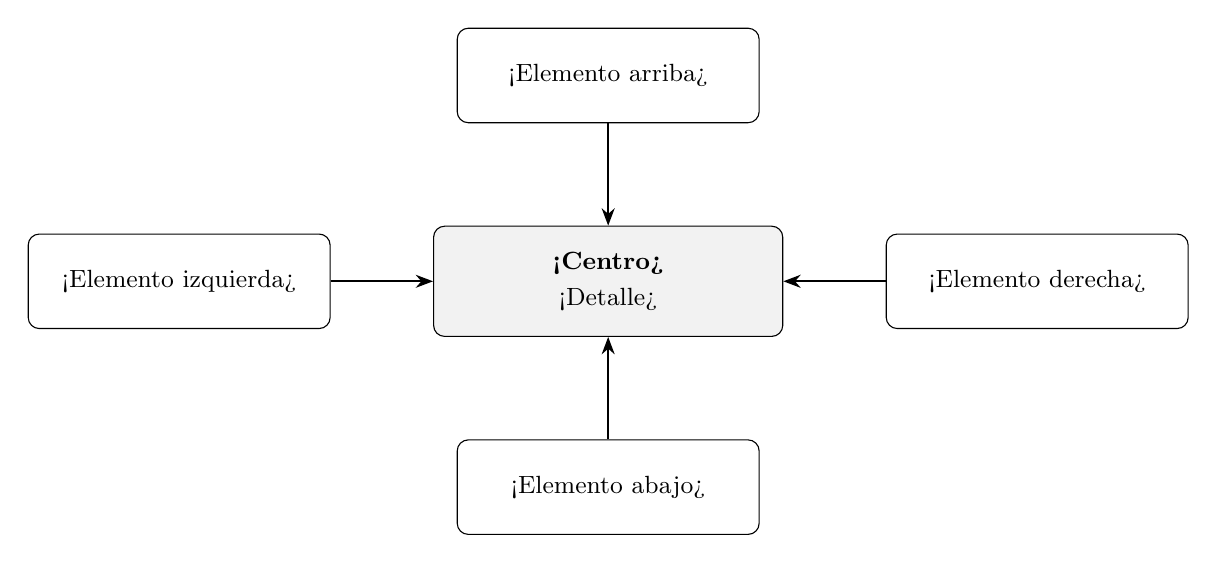
\begin{tikzpicture}[
    box/.style={draw, rounded corners, align=center, text width=3.6cm, minimum height=1.2cm, font=\small},
    centro/.style={draw, rounded corners, fill=gray!10, align=center, text width=4.2cm, minimum height=1.4cm, font=\small},
    arrow/.style={-{Stealth[length=2.2mm]}, thick}
]
\node[centro] (c) {\textbf{<Centro>}\\[2pt]<Detalle>};
\node[box, above=1.3cm of c] (a) {<Elemento arriba>};
\node[box, below=1.3cm of c] (b) {<Elemento abajo>};
\node[box, left=1.3cm of c]  (i) {<Elemento izquierda>};
\node[box, right=1.3cm of c] (d) {<Elemento derecha>};
\draw[arrow] (a) -- (c);
\draw[arrow] (b) -- (c);
\draw[arrow] (i) -- (c);
\draw[arrow] (d) -- (c);
\end{tikzpicture}
\caption{<Título de la figura>}\label{fig:radial}
\end{figure}

% ============== CONCLUSIONES ==============
\newpage
\section*{Conclusiones}
\addcontentsline{toc}{section}{Conclusiones}

\begin{itemize}
    \item <Hallazgo concreto que salga del análisis, no un resumen genérico.>
    \item <Otro hallazgo.>
\end{itemize}

% ============== REFERENCIAS ==============
\newpage
\section*{Referencias}
\addcontentsline{toc}{section}{Referencias}

\begin{hangparas}{0.5in}{1}

<Apellido, N. (Año). \textit{Título} (ed.). Editorial.>

<Entidad. (Año). \textit{Título}. \url{https://...}>

\end{hangparas}

\end{document}
